\subsection{Simulation Setup}

All algorithms run on a custom discrete-event \acrotip{VEC} simulator written in C++20 using \texttt{simcpp20} and the Armadillo linear algebra library. Neural networks are trained and exported using LibTorch (PyTorch's C++ API). Mobility scenarios are generated with realistic \acrotip{V2X} parameters, with vehicular speeds from \SI{30}{\kilo\meter\per\hour} to \SI{120}{\kilo\meter\per\hour}, \acrotip{5G} uplink bandwidth of \SI{20}{\mega\hertz}, \acrotip{V2V} sidelink of \SI{10}{\mega\hertz}, \acrotip{RSU} frequency $f_{\mathrm{RSU}} = \SI{2}{\giga\hertz}$, and on-board frequency $f_{\mathrm{loc}} \in [0.5;\, 1.0]$\,GHz. Task deadlines follow a truncated Gaussian in $[0.05;\, 2.0]$\,s; CPU complexity $C_j \sim \mathrm{Uniform}[10^8, 10^{10}]$ cycles.

\paragraph{Training.} All \acrotip{DRL} agents are trained for 400 episodes in scenarios with a fixed vehicular density of \SI{10}{tasks\per\second}. Each training episode simulates 100 task arrivals with a new mobility realization drawn from the same distribution.

\paragraph{Testing.} After training, agents are evaluated zero-shot across 601 test scenarios covering five density regimes: $\{10, 15, 20, 25, 30\}$~tasks/s. No additional learning or adaptation occurs during testing.

\paragraph{Baselines.} We compare against: Always-Local (never offloads), Greedy (always offloads to the \acrotip{V2V} pair with the lowest estimated \acrotip{JCT}, an optimistic oracle baseline), Greedy-Fair (greedy with Jain's fairness constraint), Random (offloads to a random pair), SAC-Base (\acrotip{SAC} with an 11-dimensional raw state vector, without \acrotip{TOPSIS}), PPO-TOPSIS (on-policy \acrotip{PPO} with the same 6D \acrotip{TOPSIS} state), and TD3-TOPSIS (off-policy \acrotip{TD3} with the same 6D \acrotip{TOPSIS} state).

\paragraph{Metrics.}
\begin{itemize}[nosep,leftmargin=*]
  \item \textbf{Deadline fulfillment rate}: fraction of tasks with $\mathrm{JCT}_j \le D_j$.
  \item \textbf{\acrotip{SWQ}}: $\mathrm{SWQ} = \hat{\tau} \cdot \overline{\bigl[(D_j - \mathrm{JCT}_j)/D_j\bigr]}_{\mathrm{success}}$, which rewards meeting the deadline with a large margin.
  \item \textbf{Average \acrotip{JCT}} and \textbf{total energy consumed}.
\end{itemize}

\subsection{General Performance Comparison}

Figure~\ref{fig:performance} and Table~\ref{tab:results} summarize the aggregated performance across all 601 test scenarios.

\begin{figure}[t]
  \centering
  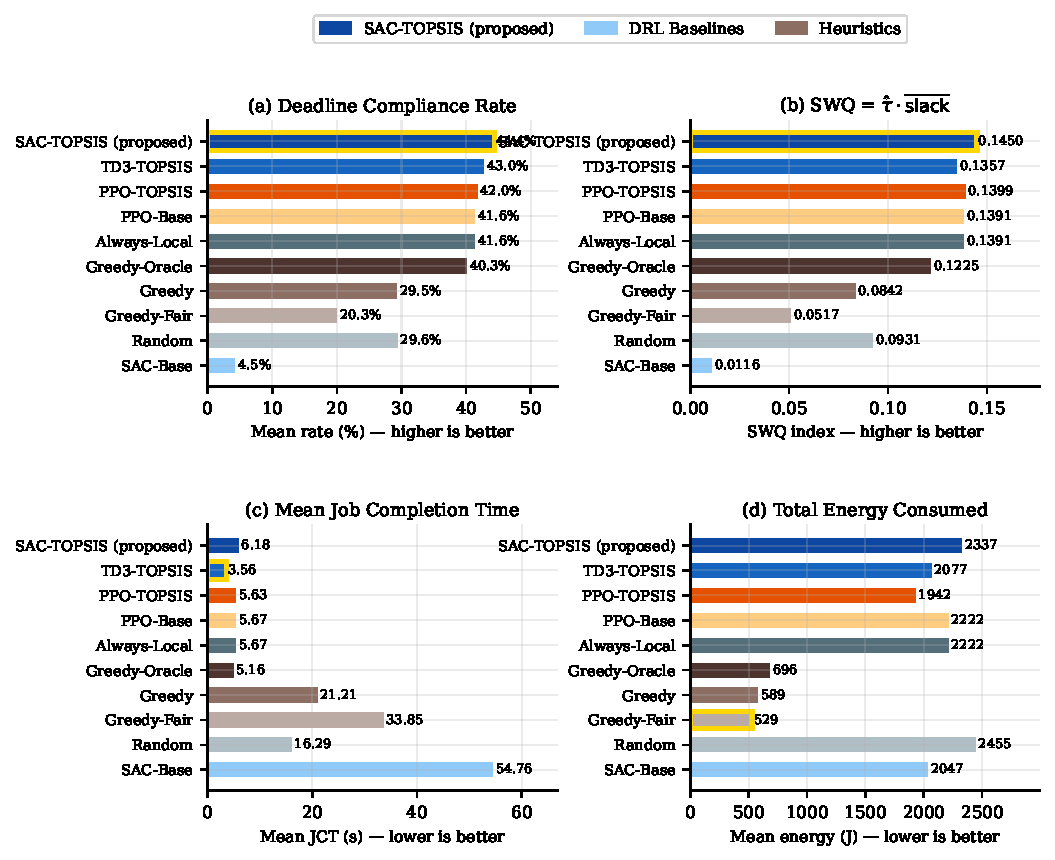
\includegraphics[width=\columnwidth]{images/fig_02_performance.pdf}
  \caption{Performance comparison across main metrics.
           \acrotip{SAC}-\acrotip{TOPSIS} (dark blue) achieves the highest deadline fulfillment rate and the highest \acrotip{SWQ} index.
           The gold border marks the best value in each chart.}
  \label{fig:performance}
\end{figure}

\begin{table}[t]
\caption{Aggregated performance across 601 test scenarios (average per scenario, densities $\{10,15,20,25,30\}$~tasks/s). Arrows ($\uparrow$) indicate the gain from adding \acrotip{TOPSIS} to each base algorithm. Bold indicates the best \acrotip{DRL} value; $\dagger$ indicates the oracle baseline.}
\label{tab:results}
{\small
\addtolength{\tabcolsep}{-3pt}
\begin{tabularx}{\linewidth}{X >{\raggedleft\arraybackslash}X >{\raggedleft\arraybackslash}X >{\raggedleft\arraybackslash}X >{\raggedleft\arraybackslash}X}
\toprule
\textbf{Policy} & \textbf{Deadline (\%)} & \textbf{\acrotip{SWQ}} & \textbf{\acrotip{JCT} (s)} & \textbf{Energy (J)} \\
\midrule
SAC-Base               &  4.47 & 0.0116 & 54.76 & 2047 \\
\acrotip{SAC}-\acrotip{TOPSIS} $\uparrow\mathbf{+39.9}$ & \textbf{44.36} & \textbf{0.1450} & 6.18 & 2337 \\
\midrule
TD3-Base               & 41.62 & 0.1391 &  \textbf{3.53} & 2222 \\
TD3-TOPSIS $\uparrow+1.4$  & 43.01 & 0.1357 &  3.56 & 2077 \\
\midrule
PPO-Base               & 41.61 & 0.1391 &  5.67 & 2222 \\
PPO-TOPSIS $\uparrow+0.3$  & 41.95 & 0.1399 &  5.63 & \textbf{1942} \\
\midrule
Always-Local           & 41.61 & 0.1391 &  5.67 & 2222 \\
\midrule
Greedy-Oracle$^\dagger$ & 40.31 & 0.1225 &  5.16 &  696 \\
Greedy                 & 29.54 & 0.0842 & 21.21 &  589 \\
Greedy-Fair            & 20.26 & 0.0517 & 33.85 &  529 \\
Random                 & 29.61 & 0.0931 & 16.29 & 2455 \\
\bottomrule
\end{tabularx}}
\end{table}

\paragraph{\acrotip{TOPSIS} consistently improves all \acrotip{DRL} families.} Table~\ref{tab:results} reveals a central result of this article: pairing \acrotip{TOPSIS} with any tested \acrotip{DRL} algorithm improves the deadline fulfillment rate relative to its corresponding base version. The magnitude of the gain, however, varies substantially across algorithm families and reflects the interaction between the \acrotip{TOPSIS} state and each algorithm's exploration strategy.

\acrotip{SAC} experiences the most dramatic improvement: SAC-Base achieves only $4.47\%$ fulfillment because it converges to an almost-always-offload policy ($94.9\%$ \acrotip{V2V}), incurring prohibitive queue delays when neighbors are congested. Adding the \acrotip{TOPSIS} state rescues the policy to $44.36\%$ ($\mathbf{+39.9}$\,pp), the best result among all evaluated policies. The 6D representation provides the semantic signal, with urgency ratios and queue occupancies, necessary for \acrotip{SAC} to distinguish beneficial from harmful offloading decisions.

\acrotip{TD3} already collapses to always-local in its base form ($41.62\%$, identical to Always-Local), as its deterministic policy avoids the risky \acrotip{V2V} path without exploration pressure. With the \acrotip{TOPSIS} state, \acrotip{TD3} learns to exploit \acrotip{V2V} opportunistically ($23.4\%$), raising fulfillment to $43.01\%$ ($+1.4$\,pp) and achieving the lowest average \acrotip{JCT} ($3.56$\,s) of all policies.

\acrotip{PPO} also collapses to always-local in its base form ($41.61\%$) due to the high variance of the on-policy gradient. The \acrotip{TOPSIS} state provides a marginal improvement to $41.95\%$ ($+0.3$\,pp). The gain is limited because \acrotip{PPO}'s on-policy nature prevents it from fully exploiting the richer state, as variance in gradient estimates still pushes the policy toward the safe local action despite the informative $s_2$ signal (offloading advantage).

Overall, \acrotip{SAC}-\acrotip{TOPSIS} achieves the highest deadline fulfillment rate ($44.36\%$) and \acrotip{SWQ} ($0.1450$) among all policies, including the Greedy oracle baseline ($40.31\%$). The results confirm that the \acrotip{TOPSIS} state is the primary performance driver, rather than the choice of \acrotip{DRL} algorithm, as all three families benefit, and the residual differences between them are side effects of their respective exploration mechanisms.

\subsection{Zero-Shot Generalization}

Figure~\ref{fig:generalization} shows the deadline fulfillment rate as a function of vehicular density. \acrotip{SAC}-\acrotip{TOPSIS} consistently leads across all densities, maintaining $>34\%$ fulfillment even in the most severe unseen congestion regime ($\SI{30}{tasks\per\second}$), where heuristic Greedy drops to only $14\%$. The difference over Always-Local ranges from $+1.73$\,pp at 25~tasks/s to $+4.15$\,pp at 10~tasks/s, confirming that the benefit of learning an adaptive policy is more pronounced in lower congestion, where opportunistic \acrotip{V2V} offloading is more reliable.

\begin{figure}[t]
  \centering
  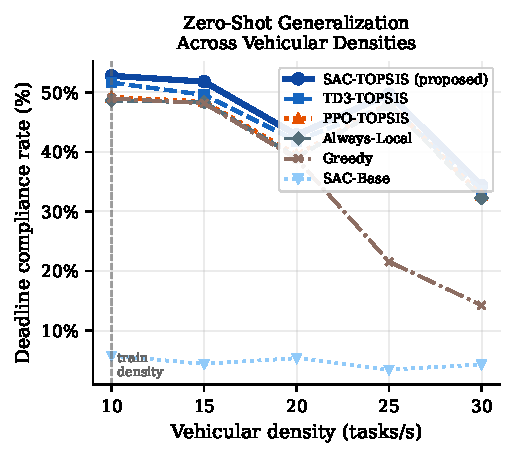
\includegraphics[width=0.75\columnwidth]{images/fig_03_generalization.pdf}
  \caption{Deadline fulfillment rate as a function of vehicular density. All agents were trained only at 10~tasks/s (dashed vertical line). \acrotip{SAC}-\acrotip{TOPSIS} (solid circles) consistently outperforms all baselines without density-specific retraining.}
  \label{fig:generalization}
\end{figure}

The scale invariance of the 6D state vector is the fundamental enabler: as $s_3$–$s_4$ are deadline-relative ratios and $s_5$–$s_6$ are normalized queue occupancies, the policy learned by the agent transfers directly to environments with more or fewer candidates. SAC-Base, in contrast, encodes absolute queue sizes and raw frequency values that lose their meaning under distribution changes.

\subsection{Execution Mode Distribution}

Figure~\ref{fig:modes} shows the average proportion of local, \acrotip{RSU}, and \acrotip{V2V} executions per policy. \acrotip{SAC}-\acrotip{TOPSIS} exploits \acrotip{V2V} offloading ($25.9\%$), which offers lower latency than \acrotip{RSU} when a peer vehicle is close. Crucially, the \acrotip{TOPSIS} module ensures that \acrotip{V2V} is chosen only when it offers a better \acrotip{TOPSIS} score than \acrotip{RSU}, preventing load migration to overloaded peers.

\begin{figure}[t]
  \centering
  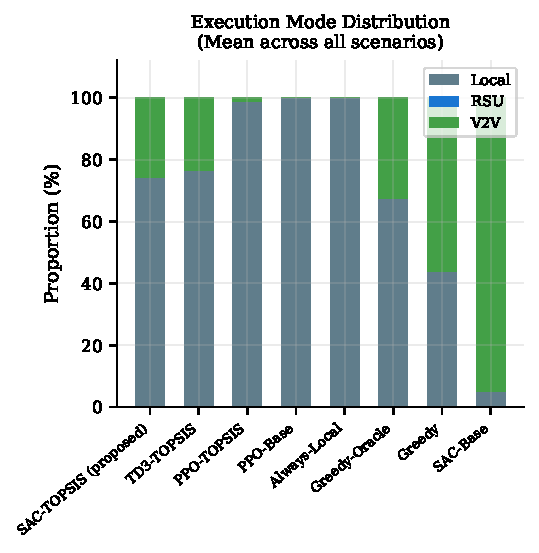
\includegraphics[width=0.75\columnwidth]{images/fig_04_modes.pdf}
  \caption{Execution mode distribution. \acrotip{SAC}-\acrotip{TOPSIS} adaptively balances local and \acrotip{V2V} execution, while SAC-Base overloads the \acrotip{RSU} with offloads.}
  \label{fig:modes}
\end{figure}

\subsection{Training Convergence}

Figure~\ref{fig:training} compares the training curves of \acrotip{SAC}-\acrotip{TOPSIS}, SAC-Base, TD3-TOPSIS, and PPO-TOPSIS. All agents are trained for 400 episodes in the 10~tasks/s scenario. \acrotip{SAC}-\acrotip{TOPSIS} and TD3-TOPSIS exhibit faster reward improvement and lower variance than SAC-Base, confirming that the \acrotip{TOPSIS} state provides a more informative learning signal. PPO-TOPSIS converges to a local optimum with lower average reward, consistent with its always-local policy at test time.

\begin{figure}[t]
  \centering
  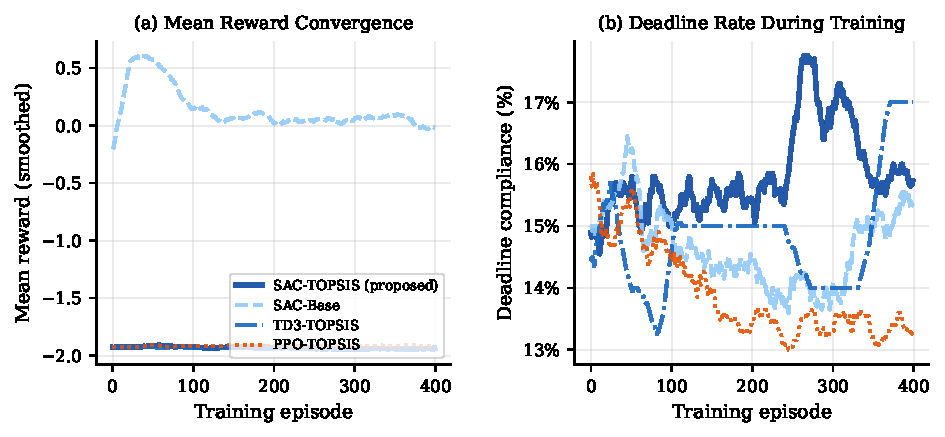
\includegraphics[width=\columnwidth]{images/fig_05_training.pdf}
  \caption{Training convergence over 400 episodes. (a) Average reward (smoothed with a 20-episode window); (b) deadline fulfillment rate during training. \acrotip{SAC}-\acrotip{TOPSIS} achieves stable convergence in both metrics.}
  \label{fig:training}
\end{figure}

\subsection{Ablation Study: \acrotip{TOPSIS} as a Universal State Engineering Primitive}
\label{sec:ablation}

Figure~\ref{fig:ablation} presents a cross-family ablation in which each \acrotip{DRL} algorithm is evaluated with its raw base state and with the 6D \acrotip{TOPSIS} state, keeping all other hyperparameters identical. The arrows annotating each pair quantify the gain attributable exclusively to the change in state representation.

Three findings stand out. First, the gain is monotonic, as \acrotip{TOPSIS} never harms any algorithm. Second, the gain is larger for the most unstable base policy (SAC-Base collapses, \acrotip{SAC}-\acrotip{TOPSIS} recovers), confirming that the \acrotip{TOPSIS} state solves the representation collapse problem rather than just fine-tuning a reasonable policy. Third, the gain is algorithm-agnostic, as even \acrotip{TD3}, which has a well-behaved (though conservative) base policy, improves by $+1.4$\,pp after the state change. This last point is fundamental, as it shows that the \acrotip{TOPSIS} state carries useful information beyond what any base algorithm can infer from raw observations, and that this information is exploitable by different learning paradigms.

\begin{figure}[t]
  \centering
  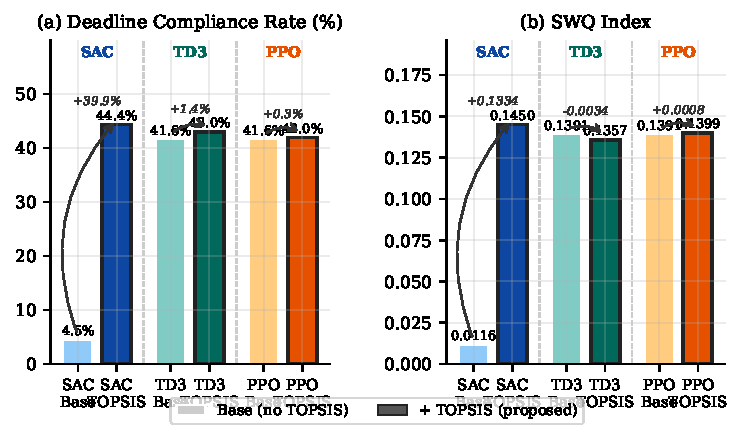
\includegraphics[width=\columnwidth]{images/fig_06_ablation.pdf}
  \caption{Cross-family ablation: Base (without \acrotip{TOPSIS}, lighter bars) vs. +\acrotip{TOPSIS} (darker bars with black border) for \acrotip{SAC}, \acrotip{TD3}, and \acrotip{PPO}. Curved arrows show the gain from adding \acrotip{TOPSIS} to each family. The gain is consistent across all families, confirming that \acrotip{TOPSIS} state compression is a universal performance driver.}
  \label{fig:ablation}
\end{figure}

\subsection{Internal \acrotip{SAC} Ablation: Causal Decomposition}
\label{sec:sac_ablation}

To understand which design choices within \acrotip{SAC}-\acrotip{TOPSIS} contribute most to its performance, we conducted a refined ablation in which each variant adds exactly one component relative to SAC-Base. Table~\ref{tab:sac_ablation} and Figure~\ref{fig:sac_ablation} summarize the results.

\begin{table}[t]
\caption{Internal \acrotip{SAC} ablation. Each row adds a design choice over SAC-Base. $\Delta$ is the gain in deadline rate relative to SAC-Base.}
\label{tab:sac_ablation}
{\small
\addtolength{\tabcolsep}{-4pt}
\begin{tabularx}{\linewidth}{X >{\centering\arraybackslash}X >{\raggedleft\arraybackslash}X >{\raggedleft\arraybackslash}X}
\toprule
\textbf{Variant} & \textbf{Change} & \textbf{Deadline} & $\boldsymbol{\Delta}$ \\
\midrule
SAC-Base  & — (base)                        &  4.47\% & —      \\
SAC-A1    & Binary action                     & 38.59\% & +34.1  \\
SAC-R1    & Reward                      & 37.64\% & +33.2  \\
SAC-S1    & Compact state                 & 28.32\% & +23.8  \\
SAC-T1    & \acrotip{TOPSIS} 3-ac           & 32.10\% & +27.6  \\
\acrotip{SAC}-\acrotip{TOPSIS}& Complete            & \textbf{44.36}\% & \textbf{+39.9}  \\
\bottomrule
\end{tabularx}}
\end{table}

\begin{figure}[t]
  \centering
  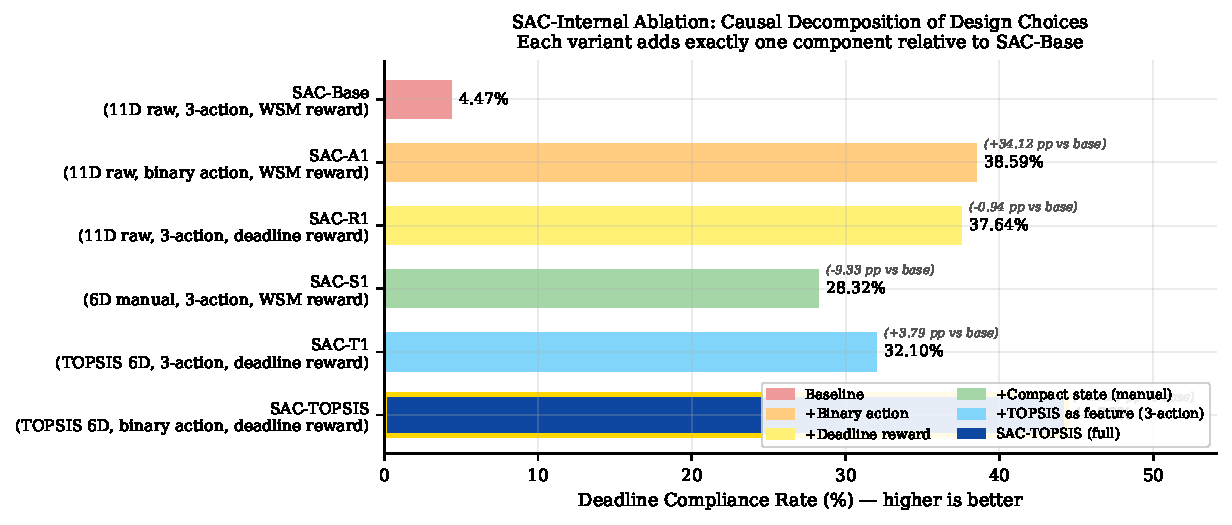
\includegraphics[width=\columnwidth]{images/fig_07_sac_ablation.pdf}
  \caption{Internal \acrotip{SAC} causal decomposition. Each bar corresponds to a variant that isolates a design choice. All gains are reported relative to SAC-Base ($4.47\%$). Complete \acrotip{SAC}-\acrotip{TOPSIS} combines all three components and achieves the highest fulfillment rate.}
  \label{fig:sac_ablation}
\end{figure}

Three complementary perspectives emerge from this decomposition.

\begin{enumerate}[label=(\arabic*),leftmargin=*]
  \item Binary action is the largest individual lever (+34.1\,pp, SAC-A1). Reducing the action space from three classes (LOCAL/\acrotip{RSU}/\acrotip{V2V}) to a binary decision (LOCAL vs. rank-1 best offloading) largely solves SAC-Base's collapse. Without \acrotip{TOPSIS}, the agent still must evaluate candidates based on raw features, but simplifying the decision boundary already prevents the degenerate always-V2V policy.
  
  \item Deadline-aware reward modeling is equally critical (+33.2\,pp, SAC-R1). Replacing Weighted Sum Method (\acrotip{WSM}) reward with continuous deadline-proportional reward from Equation~\eqref{eq:reward} provides a gradient signal even in the failure regime, allowing the agent to learn to minimize delay rather than just avoid it. This gain is independent of the state representation, demonstrating that reward engineering is an autonomous contribution.
  
  \item \acrotip{TOPSIS} state yields compound gains over any isolated component. SAC-S1 shows that manually compacting the state to 6D (without \acrotip{TOPSIS}) already yields $+23.8$\,pp over SAC-Base, confirming that feature engineering matters. SAC-T1 shows that using \acrotip{TOPSIS} to build the 6D state (instead of ad-hoc features) raises this to $+27.6$\,pp, even when the action space still has 3 classes. Complete \acrotip{SAC}-\acrotip{TOPSIS}, combining \acrotip{TOPSIS} state with binary action and deadline reward, achieves $+39.9$\,pp, more than any individual component, confirming that the three design choices are synergistic rather than merely additive.
\end{enumerate}
